\section{Optimization for Piecewise Linear Valuations} \label{sec:convex-opt-for-pwl}
In this section we show that for the case where the item space is $\Theta = [0,1]$ and the buyers' valuations $v_i$ are piecewise linear functions on $[0,1]$, it is possible to reformulate our infinite-dimensional convex program \eqref{eq:eg-primal} as a finite-dimensional convex conic program. 
This finite-dimensional program can be solved efficiently using off-the-shelf interior-point methods.
Based on the optimal solution of this reformulation, an approximate pure equilibrium allocation can be constructed easily.
This yields a highly practical approach for solving the case of piecewise linear valuations.
Unfortunately, the current theory of interior-point methods does not allows us to immediately conclude that we have a polynomial-time algorithm.
To complement our practical convex conic program, we use the ellipsoid method to 
show that there exists a theoretical algorithm that finds an $\epsilon$-approximate pure equilibrium allocation in time polynomial in $n$, $K$ and $\log \frac{\kappa}{\epsilon}$, where $\kappa$ is the inverse of the smallest buyer budget $\min_i B_i$.

As discussed in \S\ref{sec:equi-and-dual}, when all $B_i$ are equal we are in the CEEI case, and  a pure equilibrium allocation in which each buyer gets a union of intervals is a fair division in the sense of \citep{weller1985fair}. 
Hence, our method gives a polynomial-time algorithm for finding a fair division of the unit interval under piecewise linear valuations.

The key to our tractable convex conic program is to show that when the buyers' valuations $v_i$ are piecewise linear and $\Theta = [0,1]$, the set of feasible utilities $U(v, [0,1])$ defined in \eqref{eq:def-U-U(v,Theta)} can be represented by a small number of simple linear and quadratic constraints with a small number of auxiliary variables.
The first subsection shows this result for a type of normalized linear valuations on the $[0,1]$ interval. The second subsection extends the characterization to general intervals $[a,b]$ and unnormalized linear valuations, which is necessary for handling piecewise linear valuations later. 
The next two subsections show our practical and theoretical algorithmic results, respectively, followed by numerical examples and experiments.

\subsection{Characterization of the set $U(v, [0,1])$ under linear $v_i$} \label{subseq:charact-linear-vi-[0,1]}
We first characterize the set of feasible utilities when each valuation $v_i$ is \emph{linear} over the unit interval $[0,1]$. 
We will show that it can be represented by $O(n)$ linear and quadratic constraints using $O(n)$ auxiliary variables. Before proceeding, we note that, for a nonnegative linear function $v_i: \theta \mapsto c_i \theta + d_i$ on $[0,1]$, the following operations take constant time:
\begin{itemize}
	\item Eval: given $[a,b] \subseteq [0,1]$ the utility of the interval is 
	$ v_i([a,b]) = \int_a^b v_i(\theta)d\theta = \frac{c_i}{2} (b^2 - a^2) + d_i (b-a)$.
	\item Cut: given $a \in [0,1]$ and $0\leq u_0 \leq v_i([a, 1])$, finding $b\in [a,1]$ such that $v_i([a,b]) = u_0$ amounts to solving a simple quadratic equation
	$v_i([a,b]) = \frac{c_i}{2}(b^2 - a^2) + d_i(b-a) = u_0$, which gives $b = \frac{-d_i + \sqrt{d_i^2 - c_i(c_i a^2 + 2d_ia+2u_0)}}{c_i}$.
\end{itemize}
The names ``eval'' (evaluation of the utility of a given interval) and ``cut'' (finding a cut such that the utility of the resulting interval equals a given value) are customary in the cake-cutting literature \citep{procaccia2014cake,robertson1998cake}.

\paragraph{Geometry of a pure equilibrium allocation.} 
Recall that, by \cref{cor:me-structiral-properties} and \cref{eq:comp-slack-dual}, if $\{\Theta_i\}$ is a pure equilibrium allocation, then it must hold that $\Theta_i \subseteq \{p^* = \beta^*_i v_i \}$ (each buyer only gets a non-zero allocation in regions where $\beta^*_i v_i$ is the maximum among all buyers). 
When the valuations $v_i$ are linear functions on $[0,1]$, $p^*$ must be a piecewise linear (p.w.l.) function with at most $n$ pieces. 
We will use this to show that, in the case of linear valuations, a pure equilibrium allocation only needs to consist of $(n-1)$ cuts on $[0,1]$, resulting in $n$ intervals, one for each buyer. 
If we are able to compute the equilibrium utilities $u^*_i$ and an \emph{ordering} of the buyers specifying who gets the first interval starting at $0$, who gets the second interval, and so on, then an equilibrium allocation reduces to performing at most $n$ ``cut'' operations to find the exact endpoints of these intervals. 
Such an ordering of the buyers at equilibrium can in fact be determined \emph{a priori}. 
Intuitively, a buyer with a higher valuation on the left of the unit interval should always be assigned items on the left as well. 
This motivates us to consider an ordering based on the magnitudes of each valuation intercept $v_i(0) = d_i$. 
Since equilibrium allocations are invariant under arbitrary scaling of each $v_i$, such an ordering must be independent of the absolute magnitudes of buyers' valuations $\|v_i\|$. 
Hence, we consider normalized valuations such that for each $i$, $\|v_i\| = v_i([0,1]) = 1$, and we assume that the buyer indices are sorted by their intercepts $d_i$ in descending order. 
We also assume that the valuations $v_i$ are distinct. Due to normalization, this is equivalent to the intercepts $d_i$ being distinct. 

\begin{assumption}
	The item space is $\Theta = [0,1]$. 
	The valuation of each buyer $i$ is linear and nonnegative: 
	$v_i(\theta) = c_i \theta + d_i \geq 0, \, \theta\in [0,1]$.
	The valuations are normalized so that
	$v_i(\Theta) = \|v_i\| = \int_0^1 v_i(\theta) d\theta = \frac{c_i}{2} + d_i = 1$.
	The intercepts of $v_i$ are sorted in decreasing order
	$2 \geq d_1 > \dots > d_n \geq 0$.
	\label{assump:linear-distinct-decreasing-[0,1]}
\end{assumption}
The upper and lower bounds in Assumption \ref{assump:linear-distinct-decreasing-[0,1]} are due to nonnegativity: $v_i(0) \geq 0$ and $v_i(1) \geq 0$ imply $d_i \geq 0$ and $0 \leq c_i + d_i = 2(1-d_i) + d_i \Rightarrow d_i \leq 2$. The following lemma shows that, under Assumption~\ref{assump:linear-distinct-decreasing-[0,1]}, the equilibrium prices $p^*$ are p.w.l. with exactly $n$ linear pieces, corresponding to intervals that are the pure equilibrium allocations to the buyers.
\begin{lemma}
	Under Assumption~\ref{assump:linear-distinct-decreasing-[0,1]} and budgets $B_i > 0$, the equilibrium prices $p^* = \max_i \beta^*_i v_i$ are piecewise linear with exactly $n$ linear pieces.
	The (unique) breakpoints of the linear pieces $0 = a^*_0 < a^*_1 < \dots < a^*_n = 1$ induce a pure allocation: buyer $i$ receives $\Theta_i = [a^*_{i-1}, a^*_i]$, $i\in [n]$. This allocation is the unique equilibrium allocation.
	\label{lemma:all-linear-equilibrium-geometry}
\end{lemma}	
\paragraph{Recovering a pure allocation given feasible utilities.} 
Based on Lemma~\ref{lemma:all-linear-equilibrium-geometry}, we can establish Lemma~\ref{lemma:all-linear-represent-any-u} below, which ensures that partitioning the interval into $n$ subintervals is sufficient to attain any feasible utility $u\in U(v, [0,1])$.
A key fact used in the proof of Lemma~\ref{lemma:all-linear-represent-any-u} is a variant of the well-known second welfare theorem for an exchange economy with finitely many divisible items, but for our infinite-dimensional setting.
As a technical contribution, we state and prove a general second welfare theorem for the case of a continuum of items and general $L^1$ buyer valuations, which may be of independent interest. 
It states that any Pareto optimal allocation and its corresponding utilities are equilibrium allocations and equilibrium utilities of a Fisher market for some choice of buyer budgets. One technical challenge in establishing the lemma is the allocation space being a non-Euclidean Banach space. Hence, the set of feasible allocations cannot have a ``tractable'' dual space while having a nonempty interior at the same time (see Remark~\ref{remark:why-define-cp-then-prove}). 
This essentially rules out the use of a separation theorem in the allocation space, a key step in proving the classical finite-dimensional second welfare theorem. 
Instead, the proof relies on the convexity and compactness of the set of feasible utilities and the structure of an infinite-dimensional ME.
\begin{lemma} 
	\label{lemma:pareto-opt-utility-is-equil-of-some-B}
	Let each buyer $i$ have valuation $v_i \in L^1(\Theta)_+$ where $\Theta\subseteq \RR^d$ is a compact set. 
	Assume $v_i(\Theta)>0$ for all $i$.
	Let $u^\circ\in U$ be a Pareto optimal utility vector, that is, there is a Pareto optimal allocation $\{x^\circ_i\}$ such that $u^\circ_i = \langle v_i, x^\circ_i\rangle$. 
	Then, there exists $B \in \RR^n_+$ such that $\{x^\circ_i\}$ is an equilibrium allocation and $u^\circ_i$ are the corresponding equilibrium utilities of a Fisher market with $n$ buyers, each having valuation $v_i$ and budget $B_i$.
\end{lemma}
Using the above two lemmas, when $\Theta = [0,1]$ and $v_i$ are normalized linear valuations with descending intercepts $d_1\geq \dots \geq d_n$, we can show that any feasible utility vector $u\in U(v, [0,1])$ can be attained by a pure allocation of $[0,1]$ consisting of $n$ intervals (some of which can have length zero).
These intervals are allocated from left to right to buyers in the order of $1, \dots, n$.
% Note that the case of some buyers having identical intercepts $d_i$ can be easily handled by treating them as a single buyer and splitting their allocation proportionally with respect to their budgets.
\begin{lemma}
	Let $v_i(\theta) = c_i \theta+d_i$ be normalized linear valuations on $[0,1]$ (i.e. $ v_i([0,1]) = \frac{c_i}{2}+d_i = 1$) such that $2\geq d_1 \geq \dots \geq d_n \geq 0$. For any $u\in  U(v, [0,1])$, there exists $a_0 = 0 \leq a_1 \leq \dots \leq a_n = 1$ such that $v_i([a_{i-1}, a_i]) \geq u_i$ for all $i$. \label{lemma:all-linear-represent-any-u}
\end{lemma}
Suppose we are given a set of feasible utilities $u \in U(v, [0,1])$ and the valuations $v_i$ are normalized and sorted in descending order of their intercept $d_i$. 
Then, we can find the breakpoints $a_0 = 0\leq a_1 \leq \dots \leq a_n=1$ in Lemma~\ref{lemma:all-linear-represent-any-u} by performing $(n-1)$ ``cut'' operations sequentially from left to right, each time computing a new $a_i\in [a_{i-1}, 1]$ such that $v_i([a_{i-1}, a_i]) = u_i$ for $i=1, \dots, n-1$ (and setting $a_n = 1$ ensures $v_n([a_{n-1}, a_n]) \geq u_n$). Later, we will present a general version of this procedure that handles unnormalized and unsorted linear valuations on an arbitrary interval $[l,h]\subseteq [0,1]$.

\paragraph{Convex conic representation of $U(v,[l,h])$.} 
Through the next two theorems, we show that the set of feasible utilities $U(v, [l,h])$ on an interval can be represented by $O(n)$ number of linear and quadratic constraints using $O(n)$ auxiliary variables.
We start with the case of sorted and normalized (but not necessarily distinct) $v_i$ on $[0,1]$.
\begin{theorem}
	Let $v_i(\theta) = c_i \theta + d_i$, $\theta\in [0,1]$ and $v_i([0,1]) = \frac{c_i}{2}+d_i = 1$ for all $i$. 
	Let $2\geq d_1 \geq \dots \geq d_n \geq 0$. 
	Denote $\mathcal{C} = \{ (t_1,t_2)\in \RR^2: t_1^2 \leq t_2 \}$, and let
	$G_i = \left[ \begin{smallmatrix}
		d_i & c_i / 2 \\[1ex]
		-d_{i+1} & -c_{i+1}/2
 	\end{smallmatrix}\right]\in \RR^{2\times 2},\ \forall\, i\in [n-1]$.
	Then, a vector of utilities $u$ is in $U(v, [0,1])$ if and only if it is part of a feasible solution to the following constraints together with auxiliary (real) variables $z_i, w_i, s_i, t_i$:
	\begin{align*}
		& u = (u_1, \dots, u_n) \geq 0, \ \ u_1 \leq z_1, \ \ u_i \leq z_i + w_{i-1},\ \forall\, i=2, \dots, n-1,\ \ u_n \leq 1 + w_{n-1},\\
		& G_i \begin{bmatrix}
			s_i \\ t_i
		\end{bmatrix} = \begin{bmatrix}
			z_i \\ w_i
		\end{bmatrix}, \, \begin{bmatrix}
			s_i \\ t_i
		\end{bmatrix} \in \mathcal{C},\ \forall\, i \in [n-1],\ \ z_i \in [0,1],\, w_i \in [-1,0],\, z_i + w_i \geq 0,\ \forall\, i\in [n-1].
	% & z_i \in [0,1],\, w_i \in [-1,0],\, i\in [n-1].
	\end{align*} 
	Furthermore, the above constraints imply $0\leq s_i \leq 1$, $0\leq t_i \leq 1$.
	\label{thm:U-conic-rep}
\end{theorem}
The key observation used in the proof is to express the \emph{Pareto frontier} of utilities as the image of a linear transformation of the product of quadratic curves $\{(t_1, t_2): t_1^2 \leq t_2\}$.
In short, the above theorem shows that  $U$ is the first $n$ dimensions of a convex compact set in $\mathbb{R}^{n+4(n-1)}$ represented by $O(n)$ linear and quadratic constraints. 
% Next, we illustrate the derivation of the above characterization via the case of $n=2$ buyers.
% The bounds on $s_i$ and $t_i$ will be useful in the subsequent time complexity analysis of computing a pure equilibrium allocation.
% \begin{example}[Representation of \text{$U(v, [0,1])$} with $n=2$ buyers] \label{ex:2-buyers-U}
% 	Under the assumptions of Theorem~\ref{thm:U-conic-rep} (linear, normalized $v_i$ sorted by $d_i$ in descending order), let $2\geq d_1 > d_2 \geq 0$. 
% 	By Lemma~\ref{lemma:all-linear-represent-any-u}, for any feasible utilities $u \in U(v, [0,1])$, we can find $a\in [0,1]$ such that $u_i \leq v_i([0, a])$, $u_2 \leq v_2([a,1])$.  
% 	Therefore, 
% 		\[ U = U(v, [0,1]) = \left\{ (u_1, u_2)\geq 0: \exists\, a \in [0,1]\ \st u_1 \leq \frac{c_1}{2}a^2 + d_1 a,\, u_2 \leq \frac{c_2}{2}(1-a^2) + d_2(1-a)  \right\}. \]
% 	Clearly, $u\in U$ if and only if $u\geq 0$ and there exist $z_1$, $w_1$, $a$ such that
% 	\begin{align*}
% 		& u_1 \leq z_1, \ u_2 \leq 1 + w_1, \\
% 		& z_1 \leq \frac{c_1}{2} a^2 + d_1 a, \ w_1 \leq -\frac{c_2}{2} a^2 - d_2 a, \\ 
% 		& a\in[0,1].
% 	\end{align*}
% 	Since $a\in [0,1]$ and $\frac{c_i}{2} + d_i = 1$, $i=1,2$, the above inequalities imply the bounds on $(z_1, w_1)$:
% 	\begin{align*}
% 		& 0 \leq u_1 \leq z_1 \leq \frac{c_1}{2} + d_1 \leq 1, \\
% 		& -1 \leq -\frac{c_2}{2} - d_2 \leq w_1 \leq u_2 - 1 \leq \frac{c_2}{2} + d_2 - 1 = 0, \\
% 		& z_1 + w_1 = (d_1 - d_2) a + \left( (1-d_1) - (1-d_2) \right)a^2 = (d_1 - d_2) (a - a^2) \geq 0,
% 	\end{align*}
% 	where the last inequality uses $d_1 \geq d_2$ and $1 \geq a \geq a^2 \geq 0$.
% 	Therefore, $u\in U$ if and only if there exists $(z_1, w_1)$ and $a$ such that 
% 	\begin{align}
% 		\begin{split}
% 			& u_1 \leq z_1, \ u_2 \leq 1 + w_1, \\
% 			& z_1 \leq \frac{c_1}{2} a^2 + d_1 a, \ w_1 \leq -\frac{c_2}{2} a^2 - d_2 a, \ a\in[0,1], \\
% 			& 0\leq z_1 \leq 1, \ -1\leq w_1 \leq 0,\ z_1 + w_1 \geq 0.
% 			\label{eq:u1-u2-z1-w1-a-in-example}				
% 		\end{split}
% 	\end{align}
% 	Let the Pareto frontier be 
% 	\[ U^\circ = \left\{ \left( \frac{c_1}{2}a^2 + \frac{d_1}{2}, \frac{c_2}{2}(1-a^2) + \frac{d_2}{2}(1-a) \right): a\in [0,1] \right\}. \]
% 	For specific values of $d_1, d_2$, the Pareto frontier $U^\circ$ and the set $U$ are illustrated in Figure~\ref{fig:U-set-2}, where $U$ is the region bounded by the axes and $U^\circ$.
% 	The Pareto frontier is in fact the image under an affine transformation of a parabola:
% 	\[ U^\circ = (0,1) + \Gamma, \]
% 	where $\Gamma$ is a (linearly transformed) parabola segment:
% 	\begin{align*}
% 		& \Gamma = \left\{ \left( \frac{c_1}{2}a^2 + d_1 a, -\frac{c_2}{2} a^2 - d_2 a \right): a\in [0,1] \right \} = G_1 \{ (s_1, s_1^2): s_1\in [0,1] \}.
% 	\end{align*}
% 	The feasible region for $(z_1, w_1)$ given by \eqref{eq:u1-u2-z1-w1-a-in-example} can be described as follows:
% 	\[ S_1 = \conv(\Gamma) = \conv(\bar{\Gamma}) \cap T_1,\]
% 	where $\bar{\Gamma}$ is the \emph{entire} curve of $\Gamma$ ($a\in [0,1]$ in the parametric description replaced by $a\in \RR$) and 
% 	\[ T_1 = \{ (z_1, w_1)\in [0,1]\times [-1,0]: z_1 + w_1 \geq 0 \} \]
% 	is the triangular region given by the implied linear inequalities in \eqref{eq:u1-u2-z1-w1-a-in-example}.
% 	Since 
% 	\[ \bar{\Gamma} = G_1 \{(s_1, s_1^2): s_1 \in \RR \}, \]
% 	we have 
% 	\[ \conv(\bar{\Gamma}) = G_1 \conv( \{(s_1, s_1^2): s_1 \in \RR \} ) = G_1 \mathcal{C}. \]
% 	Hence, the feasible region for $(z_1, w_1)$ can be described by the linear inequalities in $T_1$ and $ (z_1, w_1) = G_1 (s_1, t_1)$, $(s_1, t_1) \in \mathcal{C}$. 
	
% 	We have arrived at all linear and quadratic constraints given in Theorem~\ref{thm:U-conic-rep} for the case of $n=2$. Furthermore, we can also verify that $S_1 = G_1 \conv( \{(s_1, s_1^2): s_1 \in [0,1] \} )$, where 
% 	\[ \conv( \{(s_1, s_1^2): s_1 \in [0,1] \} ) = \{ (s_1, t_1): 0\leq s_1 \leq 1,\, 0 \leq t_1 \leq 1,\, s_1^2 \leq t_1 \}. \]
% 	Therefore, we also know that $0\leq s_1, t_1 \leq 1$.

% 	% % Then, $U$ is the intersection of the ``lower-left'' side of $\Gamma$ and the nonnegative orthant:
% 	% \[ U = \conv(\Gamma) \cap \RR_+^2. \]
% 	% Note that $\Gamma$ is in fact a (rotate) parabola:
% 	% \[ \Gamma = (0,1) + G_1 \mathcal{C}^0, \]
% 	% where
% 	% \[ G_1 = \begin{bmatrix}
% 	% 	d_1 & \frac{c_1}{2} \\ -d_2 & - \frac{c_2}{2}
% 	% \end{bmatrix}, \ \ \mathcal{C}^0 = \{ (s_1, s_1^2): s_1\in \RR \} . \]
% 	% Hence, its convex hull is also the image of the convex hull of $\mathcal{C}^0$, which is $\mathcal{C}$, under the same linear transformation:
% 	% \[ \conv(\Gamma) = (0,1) + G_1 \conv(\mathcal{C}^0) = (0,1) + G_1 \mathcal{C}. \]
% 	% Hence, $(u_1, u_2) \in \conv(\Gamma)$ if and only if 
% 	% \[ (u_1, u_2) = (0,1) + G_1 (s_1, t_1), \ \ (s_1, t_1) \in \mathcal{C}. \]
% 	% Introducing auxiliary variables $z_1$ and $w_1$, we can rewrite $(u_1, u_2) \in U = \conv(\Gamma) \cap \RR_+^2$ as
% 	% \begin{align*}
% 	% 	& u_1 \leq z_1 \\
% 	% 	& u_2 \leq 1 + w_1 \\
% 	% 	& \begin{bmatrix}
% 	% 		z_1 \\ w_1 
% 	% 	\end{bmatrix} = G_1 \begin{bmatrix}
% 	% 		s_1 \\ t_1
% 	% 	\end{bmatrix}, \ \begin{bmatrix}
% 	% 		s_1 \\ t_1
% 	% 	\end{bmatrix} \in \mathcal{C}, \\
% 	% 	& u_1, u_2 \geq 0, \ z_1 \in [0,1], \ w_1 \in [-1, 0].
% 	% \end{align*}
% 	% Finally, notice that $0\leq s_1, t_1 \leq 1$ is implied: otherwise, it can be verified that one of $z_1$, $w_1$ must be outside their respective bounds. This can also been seen as follows: the Pareto frontier corresponds to the segment of $\Gamma$ with $\alpha\in [0,1]$, which corresponds to the image (in the $(z_1, w_1)$ space) of the linear transformation $G_1$ of the segment of $\mathcal{C}^0$ corresponding to $s_1\in [0,1]$.
% \end{example}

% \begin{figure}
% 	\centering
% 	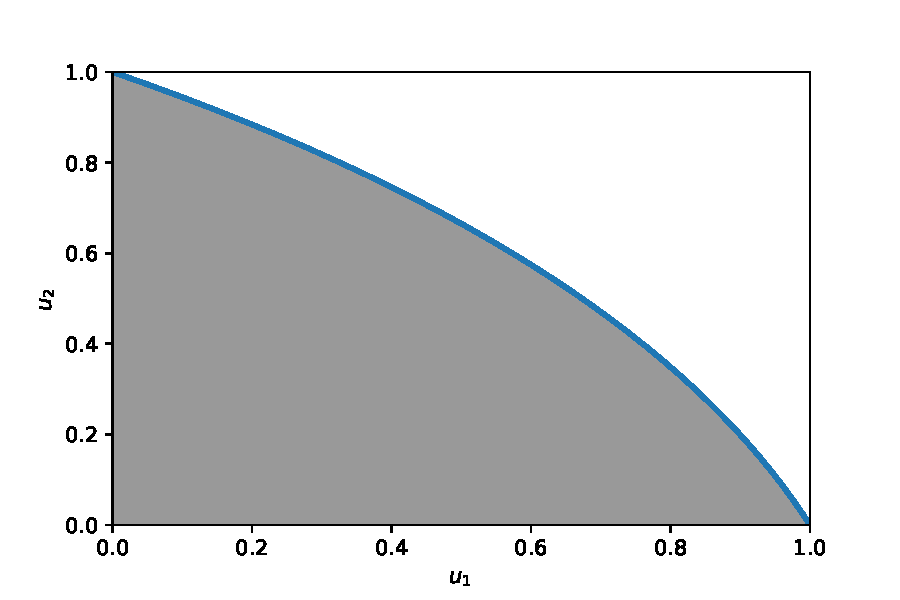
\includegraphics[scale=0.5]{codes/U-set-two-buyers.pdf}
% 	\caption{An illustration of the Pareto frontier $U^\circ$ (the curve connecting $(0,1)$ and $(1,0)$) and $U(v, [0,1])$ (the set of feasible utilities, i.e., the shaded region bounded by the Pareto frontier and two axes) in Example~\ref{ex:2-buyers-U}. Here, $d_1 = 1.5$, $d_2 = 0.8$ and $c_i = 2(1-d_i)$, $i=1,2$.}
% 	\label{fig:U-set-2}
% \end{figure}

\subsection{The case of general linear $v_i$}
When $v_i$ are defined on a general interval $[l,h]\subseteq [0,1]$ and are neither normalized nor sorted in any particular order, we can still utilize Theorem~\ref{thm:U-conic-rep} to characterize the set of feasible utilities. 
In this case, $U(v, [l,h])$ is the image of $U(v', [0,1])$ under a simple linear transformation, where $v' = (v'_1, \dots, v'_n)$ is the corresponding set of linear valuations defined on $[0,1]$ that satisfy the assumptions of Theorem~\ref{thm:U-conic-rep}, i.e., normalized and sorted in descending order of their intercepts. 
The linear transformation is the composition of a permutation (represented by a permutation matrix) and a scaling (represented by a diagonal matrix). The following theorem describes the characterization of $U(v, [l,u])$ in detail.
\begin{theorem}
	Let $v_i(\theta) = \frac{c_i}{2}\theta+d_i \geq 0$, $\theta\in [l,h]\subseteq [0,1]$. 
	Assume 
	$\Lambda_i := v_i([l,h]) = \frac{c_i}{2}(h^2 - l^2) + d_i(h-l) > 0$.
	Denote $\hat{c}_i = (h-l)^2 c_i/ \Lambda_i$, $\hat{d}_i = (h-l) (c_i l + d_i) /\Lambda_i$. Then, for each $i$, the normalized valuation
	$ \hat{v}_i(\theta) = \hat{c}_i(\theta)+\hat{d}_i$ 
	satisfies $\hat{v}_i([0,1]) = 1$.
	Let $\sigma$ be a permutation of $[n]$ that sorts $\hat{d}_i$ in descending order, i.e., $\hat{d}_{\sigma(1)} \geq \dots \geq \hat{d}_{\sigma(n)}$. 
	Let $P\in \{0,1\}^{n\times n}$ be the (inverse) permutation matrix of $\sigma$ with entries $P_{ij} = \mathbb{I}\{i = \sigma(j)\}$. 
	Let $D\in \RR^{n\times n}$ be a diagonal matrix with $D_{ii} = \Lambda_i := \frac{c_i}{2}(h^2-l^2) + d_i(h-l)$. It holds that
		 \[ U(v, [l,h]) = D P \hat{U}^\sigma = \{ DP u: u\in \hat{U}^\sigma \}, \]
	where $\hat{U}^\sigma = U(\hat{v}_{\sigma}, [0,1])$ is the set of feasible utilities given (sorted and normalized) valuations $\hat{v}_{\sigma(j)}$, $j \in [n]$ on $[0,1]$ with coefficients $\hat{c}_{\sigma(j)}, \hat{d}_{\sigma(j)}$.
	\label{thm:U-conic-rep-general-vi}
\end{theorem}
In Theorem~\ref{thm:U-conic-rep-general-vi}, the set $\hat{U}^\sigma$ satisfies the assumptions in Theorem~\ref{thm:U-conic-rep} (i.e., normalized valuations sorted by intercepts) and hence can be represented by $O(n)$ linear and quadratic constraints with $O(n)$ auxiliary variables. Therefore, so is $U(v, [l,h])$, which requires $n$ additional simple linear constraints, each only involving two utility variables $u_{\sigma(j)}$ (for the true utility) and $u'_j$ (for the utility in the permuted and normalized space).

\paragraph{Recovering a pure allocation given feasible utilities (revisited).}
In \S\ref{subseq:charact-linear-vi-[0,1]}, we showed how to find the breakpoints described in Lemma~\ref{lemma:all-linear-represent-any-u} given normalized and sorted $v_i$. 
Algorithm~\ref{alg:interval-partition-given-feasible-u} solves the more general case of unnormalized, unsorted $v_i$ defined on an arbitrary interval $[l,h] \subseteq [0,1]$. 
% Algorithm~\ref{alg:interval-partition-given-feasible-u} formalizes the steps of computing a partition $\{[l_i, h_i]: i\in [n] \}$ of $[l,h]$ given feasible $u\in U(v, [l,h])$. 
\begin{algorithm}
	\caption{Partition $[l,h]$ according to feasible utilities $u\in U(v, [l,h])$}
	\textbf{Input:} coefficients $c_i, d_i$ s.t. $v_i(\theta) = c_i\theta + d_i \geq 0$, $\theta\in [l,h]$, vector of feasible utilities $u\in U(v, [l, h])$. \\
	Compute $\Lambda_i$, $\hat{c}_i$, $\hat{d}_i$, $i\in [n]$ as in Theorem~\ref{thm:U-conic-rep-general-vi}. \\
	Find permutation $\sigma$ of $[n]$ such that $\hat{d}_{\sigma(1)} \geq \dots \geq \hat{d}_{\sigma(n)}$. \\
	Set $l_{\sigma(1)} = h_{\sigma(0)} = l$ (define $\sigma(0)  = 0$) and $h_{\sigma(n)} = h$.\\
	\textbf{For} $j = 1, \dots, n-1$:
	\begin{itemize}
		\item Set $i = \sigma(j)$ (buyer $i$ gets the $j$th interval, with left endpoint $l_i = l_{\sigma(j)} = h_{\sigma(j-1)}$).
		\item Find the right endpoint $h_i\in [l_i, h]$ such that $v_i([l_i, h_i]) = u_i$ by solving the quadratic equation (the ``cut'' operation)
		$\frac{c_i}{2}(h_i^2 - l_i^2) + d_i(h_i - l_i) = u_i$.
		\item Set $l_{\sigma(j+1)} = h_i$.
	\end{itemize}

	 \textbf{Return:} $[l_i, h_i]$, $i\in [n]$ s.t. $v_i([l_i, h_i])\geq u_i$ (which is equality for $i=\sigma(1), \dots, \sigma(n-1)$).
	\label{alg:interval-partition-given-feasible-u}
\end{algorithm}
Its running time is clearly $O(n\log n)$ due to the sorting step. 
The correctness of Algorithm~\ref{alg:interval-partition-given-feasible-u} is a direct consequence of Theorem~\ref{thm:U-conic-rep-general-vi} and Lemma~\ref{lemma:all-linear-represent-any-u}. 
In more detail, Lemma~\ref{lemma:all-linear-equilibrium-geometry} shows that we can partition $[0,1]$ according to the transformed valuations $\hat{v}_{\sigma(j)}$ and utility values $u_{\sigma(j)} / \Lambda_{\sigma(j)}$, and then to get an allocation of $[l,h]$ we linearly transform these intervals back to $[l,h]$ and assign the buyers in the same order. 
This can be done by directly dividing $[l,h]$ in the order of $\sigma$ according to the scaled intercepts $\hat{d}_i$.
% Alternatively, one can also normalized $v_i$ directly on $[l,h]$, that is, $\tilde{c}_i = c_i / v_i([l,h])$, $\tilde{d}_i = d_i/v_i([l,h])$, $\tilde{v}_i(\theta) = \tilde{c}_i \theta + \tilde{d}_i$, $\theta\in [l,h]$, $\tilde{v}_i([l,h])=1$ and sort the buyers via $\tilde{v}_i(l) = \tilde{c}_i l + \tilde{d}_i$, which gives the same permutation $\sigma$ (up to buyers having proportional valuations).

% Next, we give an example that illustrates the representation of $U(v, [l,h])$ in Theorem~\ref{thm:U-conic-rep-general-vi} as well as the execution of Algorithm~\ref{alg:interval-partition-given-feasible-u}. It is taken from Example~\ref{ex:pwl-numerical} in \S~\ref{subsec:numerical-examples} for recovering pure equilibrium allocations: the interval $[l,h]$ corresponds to the second predefined interval $[a_1, a_2]$ of the piecewise linear valuations $v_i$ in that example.
% \begin{example}
% 	[Representation of $U(v,{[l,h]})$ and Algorithm~\ref{alg:interval-partition-given-feasible-u}]
% 	Consider $n=4$ buyers with valuations $v_i(\theta) = c_i \theta + d_i\geq 0$, $\theta\in [l, h] = [0.3741, 0.8147]$. Here, the coefficients $c_i$ and $d_i$ of the valuations are
% 	\begin{align*}
% 		c &= (1.6253, -0.2604, -1.7084, 2.5419),\\
% 		d & = (-0.2972, 0.4864, 1.3919, 0.6464). 
% 	\end{align*}
% 	The normalized coefficients $\hat{c}_i$, $\hat{d}_i$ and normalizing constants $\Lambda_i = v_i([l,h])$, as in Theorem~\ref{thm:U-conic-rep-general-vi}, are
% 	\begin{align*}
% 		\hat{c} &= (1.0708, -0.3460, -2.0, 0.5192),\\
% 		\hat{d} &= (0.4646, 1.1730, 2.0, 0.7404),\\
% 		\Lambda &= (0.2947, 0.1461, 0.1659, 0.9506).
% 	\end{align*}
% 	The order of descending $\hat{d}_i$ is $\sigma = (3, 2, 4, 1)$, i.e., $\hat{d}_3 \geq \hat{d}_2 \geq \hat{d}_4 \geq \hat{d}_1$. 
% 	Therefore, the sorted arrays of $\hat{c}_i, \hat{d}_i$ are (e.g., $\hat{c}_{\sigma(1)} = \hat{c}_3 = -2.0$):
% 	\begin{align*}
% 		\hat{c}_\sigma &= (-2.0, -0.3460, 0.5192, 1.0708),\\
% 		\hat{d}_\sigma &= (2.0, 1.1730, 0.7404, 0.4646). 
% 	\end{align*}
% 	Using $\hat c,\hat d$, we get the transformed valuation $\hat{v}_{\sigma(j)}(\theta) = \hat{c}_{\sigma(j)} \theta + \hat{d}_{\sigma(j)} \geq 0$ for each $j=1,\ldots,4$, with a normalized value such that $\hat{v}_{\sigma(j)}([0,1]) = 1$. The elements of the diagonal matrix $D$ are $ D_{jj} = \Lambda_{\sigma(j)}  = v_{\sigma(j)}([l,h])$, i.e.,
% 	\begin{align*}
% 		(D_{11}, D_{22}, D_{33}, D_{44}) = (\Lambda_3, \Lambda_2, \Lambda_4, \Lambda_1) = (0.1659, 0.1461, 0.9506, 0.2947).
% 	\end{align*}
% 	The statement $U(v, [l,h]) = DP \hat{U}^\sigma$ in Theorem 
% 	\ref{thm:U-conic-rep-general-vi} is as follows:
% 	\begin{align*}
% 		u\in U(v ,[l,h]) \ \Leftrightarrow \ \exists\, u' \in \hat{U}^\sigma\ \st
% 		u_3 = \Lambda_3 u'_1, \ u_2 = \Lambda_2 u'_2, \ u_4 = \Lambda_4 u'_3,\ u_1 = \Lambda_1 u'_4.
% 	\end{align*}
% 	Here, the set $\hat{U}^\sigma$ can be represented by $O(n)$ linear and quadratic constraints with $O(n)$ auxiliary variables as in Theorem~\ref{thm:U-conic-rep}, since $\hat{v}_{\sigma(j)}$ are normalized on $[0,1]$ and $\hat{d}_{\sigma(1)} \geq \dots \hat{d}_{\sigma(4)}$. Next, suppose we are given $u\in U(v, [l,h])$ and need to find a partition of $[l,h]$ into $4$ intervals that achieve $u_i$. Here, we use $u = (0.0000, 0.0732, 0.0036, 0.5646) \in U(v, [l,h])$ (which is the equilibrium utility achieved on this interval in Example~\ref{ex:pwl-numerical}). The steps of Algorithm~\ref{alg:interval-partition-given-feasible-u} are as follows. 
% 	\begin{itemize}
% 		\item The allocation order is $\sigma = (3, 2, 4, 1)$, i.e. decreasing in $\hat{d}_i$.
% 		\item Since $\sigma(1) = 3$, set $l_3 = l$ and find $h_3 \in [l,h]$ such that $v_3([l,h_3]) = u_3 = 0.0036$. This gives $[l_3, h_3] = [0.3741, 0.3789]$. Set $l_{\sigma(2)} = l_2 = h_3 = 0.3789$. 
% 		\item For $\sigma(2) = 2$ we find $h_2 \in [l_2, h]$ such that $v_2([l_2, h_2]) = u_2$, which gives $[l_2, h_2] = [0.3789, 0.5815]$.
% 		\item Similarly, the next buyer is $\sigma(3) = 4$ and $[l_4, h_4] = [0.5815, 0.8147]$. 
% 		\item The last buyer is $\sigma(4) = 1$, which gets an empty interval ($l_1 = h_1 =  h = 0.8147$), resulting in zero utility $u_1 = 0$. 
% 	\end{itemize}
% \end{example} 

\subsection{Convex conic reformulation of \eqref{eq:eg-primal}} \label{subsec:convex-conic-reform-of-EG-pwl}
We now show how to handle the general case of piecewise linear valuations on $[0,1]$.
We first give a convex program whose variables are the utilities buyers receive from the subintervals defined by their linear pieces.
Formally, the item space is $\Theta = [0,1]$ and each $v_i$ is a p.w.l. valuation on $[0,1]$. Let the union of their breakpoints be $a_0 = 0 \leq a_1 \leq \dots \leq a_{K-1} \leq a_K = 1$. 
For each buyer $i\in [n]$ and each subinterval $k\in [K]$, $v_i$ is linear on $[a_{k-1}, a_k]$, i.e., 
$v_i(\theta) = c_{ik} \theta + d_{ik},\ \ \theta \in [a_{k-1}, a_k]$.
For each $k$, let the set of feasible utilities with item space $[a_{k-1},a_k]$ and valuations $v_i$ be $U_k := U(v, [a_{k-1}, a_k])$,
as defined in \eqref{eq:def-U-U(v,Theta)}. 
Consider the following convex program, whose variables denote how much utility each buyer $i$ receives from each linear segment $k$:
\begin{align}
	\sup_{(u_{ik}) \in \RR_+^{n\times K} } \, \sum_{i=1}^n B_i \log \left(\sum_{k=1}^K u_{ik}\right) \ \ \st (u_{1k}, \dots, u_{nk}) \in U_{k},\ \forall\,k \in [K].
	\label{eq:convex-prog-u(ik)}
\end{align}
By Theorem~\ref{thm:U-conic-rep-general-vi}, the set $U_k$ is the image of a permutation and a scaling of another set of feasible utilities spanned by normalized valuations on $[0,1]$:
\[ U_k = D^k P^k \hat{U}_k.\]
% Denote the permutation as $\sigma^k$ and the diagonal elements of $D^k$ as $D^k_{ii} = \Lambda_{ik}$.
Here, $\hat{U}_k$ is the set of feasible utilities spanned by $\hat{v}_{ik}$, where $v_{ik}$ is the restriction of $v_i$ on interval $[a_{k-1}, a_k]$ and $\hat{v}_{ik}$ (defined on $[0,1]$) are the normalized and sorted versions of $v_{ik}$ as described in Theorem~\ref{thm:U-conic-rep-general-vi}. 
We will adopt the notation of Theorem~\ref{thm:U-conic-rep-general-vi}, but since we need a set $\hat U_k$ for each piece $k$, we use an additional subscript $k$ to refer to the $k$th copy corresponding to the subinterval $[l,h] = [a_{k-1}, a_k]$.
Thus, $D^k$ is a diagonal matrix with diagonal entries $\Lambda_{ik} = v_i([a_{k-1}, a_k])$ (this corresponds to $\Lambda_i$ in Theorem~\ref{thm:U-conic-rep-general-vi} with $[l,h] = [a_{k-1}, a_k]$), $P^k$ is a permutation matrix corresponding to the permutation $\sigma^k$ that sorts $\hat{d}_{ik}$ (this corresponds to the intercepts $\hat{d}_i$ in Theorem~\ref{thm:U-conic-rep-general-vi}) in descending order. 
Both $D^k$ and $P^k$ depend on $(c_{ik}, d_{ik})$. 
The set $\hat{U}_k$ is the set of feasible utilities of normalized valuations as given in Theorem~\ref{thm:U-conic-rep}. 
We will use $(s_{ik}, t_{ik}, w_{ik}, z_{ik}, \hat{u}_{ik})$ to denote the  variables $(s_i, t_i, w_i, z_i, u_i)$ in Theorem~\ref{thm:U-conic-rep} corresponding to $\hat U_k$.

Next, we will describe how the convex program~\ref{eq:convex-prog-u(ik)} can be solved efficiently in practice using industry-grade interior-point methods.
% Denote $\mathcal{C} = \{ (t_1,t_2)\in \RR^2: t_1^2 \leq t_2 \}$, same as in Theorem~\ref{thm:U-conic-rep}. 
To that end, denote the $3$-dimensional second-order (quadratic) cone as $\mathcal{L} = \{ (t_1, t_2, t_3): t_1 \geq \sqrt{t_2^2+t_3^2} \}$ and the $3$-dimensional exponential cone $\mathcal{E}$ as the \textit{closure} of the following set (see, e.g., \cite{chares2009cones}): 
\[ \mathcal{E}  = \left\{ (t_1, t_2, t_3): e^{t_3/t_2} \leq t_1/t_2,\, t_2 >0 \right\}. \]
Define the following standard-form convex conic program \citep{skajaa2015homogeneous,dahl2019primal,nemirovski2004interior}:
\begin{align}
	\begin{split}
		f^* = \min\ c^\top x \ \st \ Ax = b,\,  x\in \mathcal{K}:= \RR_+^{n_1} \times \mathcal{L}^{n_2} \times \mathcal{E}^{n_3}
	\end{split} \label{eq:conic-std-form}
\end{align}
where $A\in \RR^{m\times \bar{n}}$, $c\in \RR^{\bar{n}}$, $b\in \RR^m$, $\bar{n} = n_1 + 3n_2 + 3n_3$ (we use $\bar{n}$ to denote the dimension to distinguish it from $n$, the number of buyers). 
Problem \eqref{eq:convex-prog-u(ik)} can be reformulated into \eqref{eq:conic-std-form} via standard techniques. 
The following lemma summarizes the facts about the said reformulation. 
In additional to the small dimensions $\bar{n} = O(nK)$, $m=O(nK)$, the reformulation also ensures ${\rm nnz}(A) = O(\bar{n})$, where ${\rm nnz}(A)$ denotes the number of nonzeros in the matrix $A$. A complete convex conic reformulation can be found in the proof of the lemma.
\begin{theorem}
	The supremum of \eqref{eq:convex-prog-u(ik)} is attained and is equal to $z^*$, the supremum of \eqref{eq:eg-primal}.
	For any optimal solution $(u^*_{ik})$ of \eqref{eq:convex-prog-u(ik)}, $u^*_i := \sum_{k=1}^K u^*_{ik}$ is the equilibrium utility of buyer $i$. 
	Each interval $[a_{k-1}, a_k]$ can be divided into $n$ a.e.-disjoint subintervals $[l_{ik}, h_{ik}]$ such that $u^*_{ik} = v_i([l_{ik}, h_{ik}])$. Hence, $\Theta_i := \cup_{k=1}^K [l_{ik}, h_{ik}]$, $i\in[n]$ is an equilibrium allocation. 
	Problem \eqref{eq:convex-prog-u(ik)} can be reformulated into the standard form \eqref{eq:conic-std-form} with dimensions $n_1 = O(nK)$, $n_2 = O(nK)$, $n_3 = O(n)$, $m = O(nK)$ and ${\rm nnz}(A) = O(nK)$. The minimum of the reformulation is $f^* = -z^*$.
	An optimal solution of the reformulation contains an optimal solution of \eqref{eq:convex-prog-u(ik)}, that is, $(u_{ik})\in \RR_+^{n\times K}$ such that $(u_{1k}, \dots, u_{nK})\in U_k$ for all $k$ and $\sum_k u_{ik} = u^*_i$ for all $i$.
 	 \label{lemma:eg=>u(ik)-facts}
\end{theorem}

\paragraph{Solving \eqref{eq:conic-std-form} using an interior-point method.}
The standard-form problem \eqref{eq:conic-std-form}, in which $\mathcal{K}$ is the product of a nonnegative orthant, second-order cones, and exponential cones, can be solved via off-the-shelf optimization software based on interior-point methods even for very large instances using the \emph{Mosek} solver~\citep{mosek2010mosek,dahl2019primal}. In fact, modern optimization software usually do not require such a standard-form input and allows more general input formats.
% In particular, the commercial solver Mosek \citep{mosek2010mosek,dahl2019primal} is based on a primal-dual path-following method applied to the so-called homogeneous self-dual embedding.
Although the theoretical time complexity of interior-point methods for a general convex optimization problem with computable self-concordant barrier functions has been well-studied (see e.g. \citep{nesterov1994interior}, \citep[\S 5]{nesterov2018lectures}, \citep[\S 4]{nemirovski2004interior}), to the best of our knowledge, clear-cut polynomial-time complexity results are only available for the case of \emph{self-scaled} cones, that is, linear programming (LP), second-order cone programming (SOCP) and semidefinite programming (SDP).
% via running a \emph{primal-dual path-following method} (see, e.g., \cite[\S 4.6]{ben2019lectures}). 
For general convex optimization beyond self-scaled cones, there exist bounds on the number of Newton iterations that are roughly of the form ``$O\left(\sqrt{\nu}\log \frac{M}{\epsilon}\right)$''---where $\nu$ is the barrier parameter, $\epsilon$ is the tolerance level (for duality gap and infeasibility) and $M$ is an instance-dependent constant---for ``theoretical versions'' of various interior-point methods applied to strictly feasible problems (see, e.g., \cite[\S3 and \S6]{nesterov1994interior}, \cite[5.3.4]{nesterov2018lectures}, \cite[\S 4 and \S 7]{nemirovski2004interior}).
% In the various forms of this type of bound, the constant $M$ depends critically on the geometry of the problem and the instance data, such as closeness of the initial solution to the boundary of the feasible region~\citep[Theorems~4.5.1 and 7.4.1]{nemirovski2004interior}. 
% Whether we can extend the polynomial time complexity results for self-scaled cones to the case of exponential cones is beyond the scope of this work. 
% For our purpose, it remains a challenge to bound this constant using the market data $B_i$, $c_{ik}$, $d_{ik}$ as well.  
% Furthermore, we point out that mature interior-point optimization software rarely implements all components of a theoretically-convergent method. 
% Instead, highly sophisticated numerical linear algebra methods and stepsizing heuristics are used to speed up and stabilize the computation of search directions (see e.g. \citep{toh2012implementation,sturm1999using}). These techniques, necessary for practically efficient implementations, often invalidate the theoretical complexity guarantees \citep{dahl2019primal,skajaa2015homogeneous}. 
% In conclusion, at this time one cannot derive polynomial-time solvability of the piecewise linear problem directly from our conic reformulation in~\eqref{eq:conic-std-form}.
Nevertheless, we remark that solving the reformulation~\eqref{eq:conic-std-form} of~\eqref{eq:convex-prog-u(ik)} using industry-grade interior-point optimization software (such as Mosek) is a highly efficient and stable approach for computing a pure equilibrium allocation: Mosek easily solves problems with hundreds of variables and constraints.
After computing an optimal solution $(u^*_{ik})$ of \eqref{eq:convex-prog-u(ik)} using Mosek, a pure allocation that attains these utilities can easily be found with Algorithm~\ref{alg:interval-partition-given-feasible-u}. %to divide each $[a_{k-1}, a_k]$ into subintervals among the buyers.

\subsection{A polynomial-time ellipsoid algorithm} \label{subsec:compute-pure-eq-alloc-poly-time}
Due to the problems mentioned in the previous section regarding polynomial-time solvability of conic programs involving exponential cones, we next investigate polynomial-time solvability of our problem via alternative methods.
The results in this section are primarily of theoretical interest; in practice solving the conic program from the previous section using an interior-point solver is extremely efficient and preferable.

We are going to present an algorithm that finds an $\epsilon$-approximate pure equilibrium allocation in $\poly\left(n,k,\log \frac{1}{\epsilon}\right)$ time.
This method computes approximate equilibrium utility prices using the ellipsoid method for convex optimization and constructs a pure allocation via Algorithm~\ref{alg:interval-partition-given-feasible-u}. Recall our assumptions that $\|B\|_1 = 1$ and $v_i([0,1]) = 1$ for all $i$; the unit interval is divided into $K$ subintervals by breakpoints $a_0 = 0 < a_1 < \dots < a_K = 1$; for each $i$, buyer $i$'s valuation is $v_i(\theta) = c_{ik}\theta+d_{ik}$ on the $k$th subinterval $[a_{k-1}, a_k]$. 
% We use $\beta^*$ to denote the equilibrium utility prices (see, e.g., Theorem~\ref{thm:eg-gives-me} and Lemma~\ref{lemma:beta-dual-attain}). By Lemma~\ref{lemma:beta-dual-attain} and Theorem~\ref{thm:eg-gives-me}, we know that $\beta^*$ is the unique optimal solution of problem \eqref{eq:eg-dual-beta-1}, which gives the (a.e.-unique) equilibrium prices $p^* = \max_i \beta^*_i v_i$. By Lemma~\ref{lemma:equi-bounds}, we can add the bounds $B_i \leq \beta^*_i \leq 1$ into \eqref{eq:eg-dual-beta-1} without affecting its optimal solution $\beta^*$.
\paragraph{The ellipsoid method for convex optimization.}
First, we describe the ellipsoid method for generic convex optimization \citep{shor1977cut,yudin1976informational,yudin1976evaluation,Nemirovski1977optimization}. 
We refer the readers to the survey \citep{bland1981ellipsoid} for the history of development of ellipsoid methods and further references. 
Here, we adopt the exposition in \citep{ben2019lectures}.
Consider the following generic convex program \citep[\S 4.1.4]{ben2019lectures}:
\begin{align}
	f^*:= \min_x f(x) \ \st x\in X \label{eq:generic-constrained-minimization}
\end{align}
where $f$ is convex and continuous (and hence subdifferentiable) on a compact region $X\subseteq \RR^n$.
Assume we have access to the following oracles:
\begin{itemize}
	\item The \emph{separation} oracle $\mathcal{S}$: given any $x\in \RR^n$, either report $x\in \interior X$ or return a $g\neq 0$ (representing a separating hyperplane) such that $\langle g, x\rangle \geq \langle g, y\rangle$ for any $y\in X$. 
	\item The \emph{first-order} or \emph{subgradient} oracle $\mathcal{G}$: given $x\in \interior X$ (the interior of $X$), return a subgradient $f'(x)$ of $f$ at $x$, that is, $f(y) \geq f(x) + \langle f'(x), y-x\rangle$ for any $y$.
\end{itemize} 
The time complexity of the ellipsoid method is as follows.
\begin{theorem} \cite[Theorem 4.1.2]{ben2019lectures}
	Let 
	\[V = \max_{x\in X} f(x) - f^*,\ \ R = \sup_{x\in X} \|x\|,\] and $r>0$ be the radius of a Euclidean ball contained in $X$.
	For any $\epsilon>0$, a solution $x_\epsilon\in X$ such that $f(x_\epsilon) \leq f^* + \epsilon$ can be computed using no more than $N(\epsilon)$ calls to $\mathcal{S}$ and $\mathcal{G}$, followed by no more than $O(1)n^2 N(\epsilon)$ arithmetic operations to process the outputs of the oracles, where 
	$N(\epsilon) = O(1) n^2 \log \left( 2+ \frac{V R}{\epsilon r} \right)$.
	\label{thm:4.1.2-ellipsoid-bn-notes}
\end{theorem}
Using Theorem~\ref{thm:4.1.2-ellipsoid-bn-notes}, we establish the following guarantees regarding solving \eqref{eq:convex-prog-u(ik)}.
\begin{theorem}
	For any $0 < \epsilon < 1$, we can compute $(u_{ik})\in \RR_+^{n\times K}$ such that 
	\begin{align*}
		(u_{1k}, \dots, u_{nk})\in U(v, [a_{k-1}, a_k]),\ \forall\, k\in [K], \ \  u_i := \sum_i u_{ik} \geq u^*_i - \epsilon, \ \forall\, i \in [n]
	\end{align*}
	in $O\left( n^4 K \left( \log(nK) + \log \frac{\kappa}{\epsilon} \right) \right)$ time, where $\kappa = \frac{1}{\min_i B_i}$.
	Furthermore, a pure equilibrium allocation $\{\Theta_i\}$, where buyer $i$ receives an allocation $\Theta_i = \cup_k [l_{ik}, u_{ik}]$ of at most $K$ intervals,
	% such that $[l_{ik}, u_{ik}]\subseteq [a_{k-1}, a_k]$ are a.e.-disjoint, 
	with value $v_i(\Theta_i) \geq u^*_i - \epsilon$,
	can be constructed in $O(nK)$ additional time. 
	\label{thm:ellipsoid-method-for-u(ik)-convex-program}
\end{theorem}
At a high level, in order to use Theorem \ref{thm:4.1.2-ellipsoid-bn-notes} to solve our problem \eqref{eq:convex-prog-u(ik)} in polynomial time, we need to cast it into the form \eqref{eq:generic-constrained-minimization}, construct efficient separation and first-order oracles, and bound the ratio $\frac{VR}{\epsilon r}$. To this end, all variables involved have absolute values bounded above by either absolute constants or $\kappa$. In order to ensure a nonzero radius $r>0$ of the feasible region, we can simply ``$\epsilon$-perturb'' the linear constraints and then ``$\epsilon$-discount'' the solution obtained to ensure feasibility w.r.t. the original constraints.

We remark that the constant $\kappa$ in Theorem~\ref{thm:ellipsoid-method-for-u(ik)-convex-program} can be viewed as a ``condition number'' of problem \eqref{eq:convex-prog-u(ik)}: given a fixed accuracy level $\epsilon$, the running time of the algorithm scales logarithmically (via the term $\log \kappa$) as $\kappa$ grows. 
This aligns with our intuition about a ``second-order'' method such as an interior-point method or the ellipsoid method. 
In contrast, the running time of a first-order method---such as projected gradient descent---usually scales polynomially in the problem's condition number.

\subsection{Numerical examples and experiments} \label{subsec:numerical-examples}
To round out this section, we describe two specific examples of computing a pure equilibrium over $[0,1]$ given linear and piecewise linear valuations, respectively. 
Then, we run our proposed method end-to-end on randomly generated large instances to demonstrate its scalability. 
% More details can be found in the Appendix. 

\begin{example}
	[Linear $v_i$]
	\label{ex:linear-numerical}
	Let there be four buyers with budgets $B = (0.1, 0.3, 0.2, 0.4)$ and normalized linear $v_i$ with intercepts $d = (1.2, 0.6, 0.3, 1.9)$, which implies $c = (-0.4,  0.8,  1.4, -1.8)$. Ordering the buyers by decreasing intercept gives $\sigma = (4, 1, 2, 3)$. 
	Figure~\ref{fig:n-linear} illustrates the equilibrium prices $p^*$ and the scaled valuation $\beta^*_i v_i$ for each buyer. Buyer $4$ receives the leftmost interval $[0, 0.3713]$, buyer $1$ receives $[0.3713, 0.4921]$, and so on. 
	For each buyer, its allocated interval $[l_i,h_i]$ is precisely the segment where it ``wins'', i.e., $[l_i, h_i] = \{p^* = \beta^*_i v_i\}$. 
	Since all buyers have distinct $d_i$ and positive budgets, this is the unique pure allocation. 
	% The fact that this pure allocation is indeed an equilibrium allocation (with the corresponding $\beta^*$) can also be verified using Corollary~\ref{cor:check-pure-alloc-ME}.
\end{example}


\begin{example}
	[Piecewise linear $v_i$] \label{ex:pwl-numerical}
	Let there be $n=4$ buyers, each with piecewise linear valuations $v_i$ with $K = 3$ pieces. Each buyers' linear pieces share endpoints $0 = a_0 < a_1 < a_2 < a_3 = 1$, with $a_1 = 0.3741$, $a_2 = 0.8147$. 
	Solving the convex program \eqref{eq:convex-prog-u(ik)} gives equilibrium utilities $u^*_{ik}$ for all $i,k$, where $u^*_{ik}$ is the amount of utility buyer $i$ gets from segment $[a_{k-1}, a_k]$ (which can be $0$ for some buyer-segment pairs). 
	Similarly to the linear case above, we divide each segment  $[a_{k-1}, a_k]$ among the buyers according to their $u^*_{ik}$ and their ordering according $\hat{d}_i$  on interval $k$ (c.f. Lemma~\ref{lemma:all-linear-represent-any-u}).
	%Here, since it is possible that $u^*_{ik} = 0$, a buyer may not receive an empty interval from $[a_{k-1}, a_k]$. 
	In the final pure allocation, each buyer $i$ gets a union of at most $K$ intervals, one from each $[a_{k-1}, a_k]$, which is a subset of its winning set $\{p^* = \beta^*_i v_i\}$. 
	% Each buyer's allocation $\Theta_i$ is a union of at most $K$ intervals. 
	The solution is illustrated in Figure~\ref{fig:n-pwl} using $\beta^*_i v_i$ and $p^*$.
	For example, on $[a_0, a_1]$, since $p^* > \beta^*_3 v_3$ everywhere on the segment, buyer $3$ does not get allocated anything from this interval, and thus $u^*_{31} = 0$. The same is true for buyer $4$ on $[a_0, a_1]$. 
\end{example}

\begin{figure}
\begin{minipage}{0.48\textwidth}
	\centering
	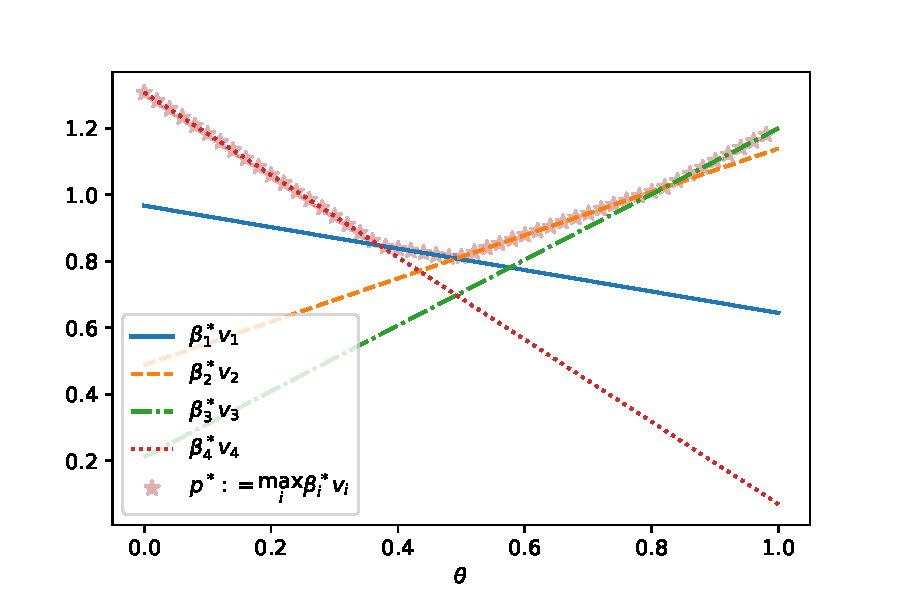
\includegraphics[scale=0.5]{codes/n-linear.pdf}
	\caption{The equilibrium prices $p^*$ and $\beta^*_i v_i$ for $4$ buyers with linear (normalized) $v_i$ on $[0,1]$ (Example \ref{ex:linear-numerical}). 
	The stars denote $p^*$, whose linear pieces correspond to the winning segments for each buyer.
	}
	\label{fig:n-linear}
\end{minipage}\hfill
\begin{minipage}{0.48\textwidth}
	\centering
	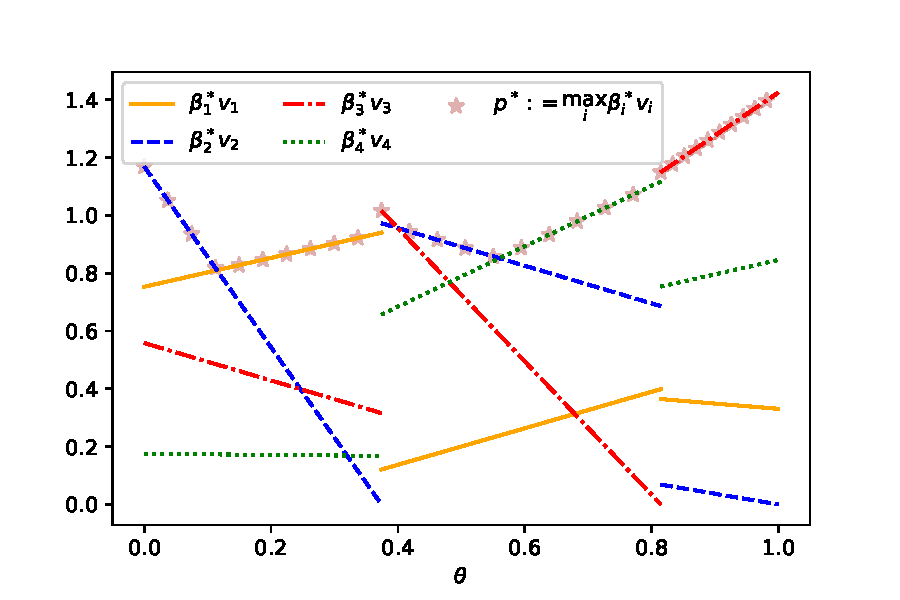
\includegraphics[scale=0.5]{codes/n-pwl.pdf}
	\caption{The equilibrium prices $p^*$ and $\beta^*_i v_i$ for $n=4$ buyers with piecewise linear $v_i$ on $[0,1]$ (Example \ref{ex:pwl-numerical}). The stars denote $p^*$, whose linear pieces correspond to the winning segments for each buyer.
	Note that each $v_i$, and hence $p^*$, are p.w.l. They are not necessarily continuous.}
	\label{fig:n-pwl}
\end{minipage}
\end{figure}

\paragraph{Large-scale experiments.} 
Next, we generate random instances with varying values of $n$ and $K$.
For each $(n,K)$ combination and each random seed value in $\{ 1, \dots, 8\}$, we perform the conic reformulation, solve the resulting convex program using Mosek and construct pure allocations based on the solution $(u^*_{ik})$.
For each $(n,K)$ combination, we record the mean running time and the standard error.
The results are presented in Table \ref{table:running-times-n-K-seeds}. 
As can be seen, for fixed $n$, the running time scales approximately linearly in $K$, and similarly running time scales linearly with $n$ for a fixed $K$. Thus our model should be scalable to very large instances.
We remark that, in the experiment, around $2/3$ of the running time arises from ``model building'', that is, constructing the sparse matrices and interacting with Mosek through its API, even after writing a highly vectorized implementation. 
Only around $1/3$ of the time arises from ``optimization'', that is, running the interior-point method through \texttt{Model.solve()}. The time for constructing pure allocations from $(u^*_{ik})$ is negligible compared to model building and computation. As an additional note for practitioners, we also tried the CVXPY modeling language: it was vastly slower at reformulating the model before calling Mosek.

% \yuan{Less significant digits.}
\begin{table}
	\begin{center}
		\begin{tabular}{|c||*{4}{c|}}\hline
\backslashbox{$n$}{$K$}
& $50$ & $100$ & $150$ & $200$\\ \hline \hline
50 & $1.53 \pm 0.05$ & $3.29 \pm 0.14$ & $5.57 \pm 0.91$ & $6.49 \pm 0.18$\\ \hline
100 & $3.34 \pm 0.14$ & $6.50 \pm 0.20$ & $10.36 \pm 0.40$ & $13.62 \pm 0.48$\\ \hline
150 & $4.84 \pm 0.12$ & $9.86 \pm 0.18$ & $16.68 \pm 1.46$ & $20.50 \pm 0.22$\\ \hline
200 & $6.44 \pm 0.07$ & $13.18 \pm 0.23$ & $20.12 \pm 0.33$ & $28.65 \pm 1.14$\\ \hline
\end{tabular}
		\caption{Running times for each $(n,K)$, mean and standard error across $8$ seeds} 
		\label{table:running-times-n-K-seeds}
	\end{center}
\end{table}